% Full instructions available at:
% https://github.com/elauksap/focus-beamertheme

\documentclass{beamer}
\usetheme[numbering=progressbar]{focus}
\usepackage{tikz}
\usetikzlibrary{positioning}
\usetikzlibrary{shapes,arrows}
\usepackage{transparent}
\usepackage{fancyvrb}
\usepackage{listings}
\usepackage{tabularx}
\definecolor{main}{RGB}{47, 161, 219}
\definecolor{background}{RGB}{240, 247, 255}
\definecolor{textcolor}{RGB}{85, 87, 83}

\title{D4 Project}
\subtitle{Open and collaborative network monitoring}
\author{Jean-Louis Huynen}
\titlegraphic{\includegraphics[scale=0.20]{../../logos/d4-logo.pdf}}
\institute{Team CIRCL \\ \url{https://www.d4-project.org/}}
\date{2019/05/21}

\begin{document}
    \begin{frame}
        \maketitle
    \end{frame}

\begin{frame}
        \frametitle{Problem statement}
        \begin{itemize}
                \item CSIRTs (or private organisations) build their {\bf own honeypot, honeynet or blackhole monitoring network}
                \item Designing, managing and operating such infrastructure is a tedious and resource intensive task
                \item {\bf Automatic sharing} between monitoring networks from different organisations is missing
                \item Sensors and processing are often seen as blackbox or difficult to audit

        \end{itemize}
\end{frame}


\begin{frame}
 \frametitle{Objective}
 \begin{itemize}
         \item Based on our experience with
           MISP\footnote{\url{https://github.com/MISP/MISP}} where sharing
           played an important role, we transpose the model in D4 project
         \item Keeping the protocol and code base {\bf simple and minimal}
         \item Allowing every organisation to {\bf control and audit their own sensor network}
         \item Extending D4 or {\bf encapsulating legacy monitoring protocols} must be as simple as possible
         \item Ensuring that the sensor server has {\bf no control on the sensor} (unidirectional streaming)
         \item Don't force users to use dedicated sensors and allow {\bf flexibility of sensor support} (software, hardware, virtual)

 \end{itemize}
\end{frame}


\begin{frame}
        \frametitle{(short) History}
 \begin{itemize}
        \item D4 Project (co-funded under INEA CEF EU program) started - 1st November 2018
        \item D4 encapsulation protocol version 1 published  - 1st December 2018
        \item v0.1 release of the D4 core\footnote{\url{https://www.github.com/D4-project/d4-core}} including a server and simple D4 C client - 21st January 2019
        \item First version of a golang D4 client\footnote{\url{https://www.github.com/D4-project/d4-goclient/}} running on ARM, MIPS, PPC and x86 - February 2019
 \end{itemize}
\end{frame}

\begin{frame}
        \frametitle{(short) History}
\begin{center}
  \begin{tabularx}{\linewidth}%
    {>{\setlength\hsize{0.6\hsize}\raggedright}X%
     >{\setlength\hsize{0.4\hsize}\raggedright}X}

\hline
Release                          & Date \tabularnewline
\hline
analyzer-d4-passivedns-v0.1      & Apr. 5,  2019 \tabularnewline
analyzer-d4-passivessl-0.1       & Apr. 25, 2019 \tabularnewline
analyzer-d4-pibs-v0.1            & Apr. 8, 2019  \tabularnewline
BGP-Ranking-1.0                  & Apr. 25, 2019 \tabularnewline
d4-core-v0.1                     & Jan. 25, 2019 \tabularnewline
d4-core-v0.2                     & Feb. 14, 2019 \tabularnewline
d4-core-v0.3                     & Apr. 8, 2019  \tabularnewline
d4-goclient-v0.1                 & Feb. 14, 2019 \tabularnewline
d4-goclient-v0.2                 & Apr. 8, 2019  \tabularnewline
d4-server-packer-0.1             & Apr. 25, 2019 \tabularnewline
IPASN-History-1.0                & Apr. 25, 2019 \tabularnewline
sensor-d4-tls-fingerprinting-0.1 & Apr. 25, 2019 \tabularnewline
\hline

\end{tabularx}
\end{center}

\end{frame}

\begin{frame}
\frametitle{D4 Overview}
        \includegraphics[scale=0.38]{../../diagram/d4-overview.png}
        % HERE there will be a timeline - not done in Tkiz
\end{frame}

\begin{frame}
        \frametitle{Roadmap}
        \begin{itemize}
          
                \item CIRCL will host an instance for organisations willing to
                  contribute without running their own D4 server, as well as for free-riders:

                  \begin{itemize}
                  \item Passive DNS collector / analyzer / lookup service
                  \item Passive SSL collector / analyzer / lookup service
                  \end{itemize}
                \item Closely followed by: 
                  \begin{itemize}
                  \item Backscatter DDoS traffic analyzer
                  \end{itemize}
        \end{itemize}
\end{frame}

\begin{frame}
\frametitle{D4 Overview}


\end{frame}




\begin{frame}
        \frametitle{D4 encapsulation protocol}
        \includegraphics[scale=0.38]{../../diagram/d4-protocol-encapsulation.png}
\end{frame}

\begin{frame}
    \frametitle{D4 Header}
    \begin{tabular}{|l|l|l|}
        \hline
        Name & 	bit size&  	Description\\
        \hline
        version &	uint 8 &	Version of the header \\
        type 	& uint 8   &	Data encapsulated type\\
        uuid 	& uint 128 & 	Sensor UUID\\
        timestamp &  	uint 64 &	Encapsulation time\\
        hmac 	& uint 256 &	Authentication header (HMAC-SHA-256-128)\\
        size 	& uint 32 	& Payload size\\
        \hline
    \end{tabular}
\end{frame}


\begin{frame}
    \frametitle{D4 Header}
    \framesubtitle{Types}
        \begin{tabular}{|l|l|}
            \hline
            Type &	Description\\
            \hline
            0 	& Reserved\\
            1 	& pcap (libpcap 2.4)\\
            2 	& meta header (JSON)\\
            3 	& generic log line\\
            4 	& dnscap output\\
            5 	& pcapng (diagnostic)\\
            6 	& generic NDJSON or JSON Lines\\
            7 	& generic YAF (Yet Another Flowmeter)\\
            8  	& passivedns CSV stream\\
            254 &	type defined by meta header (type 2)\\
            \hline
        \end{tabular}
\end{frame}

\begin{frame}
    \frametitle{D4 meta header}
    \framesubtitle{Meta types}
        D4 header includes an easy way to {\bf extend the protocol} (via type 2) without altering the format. Within a D4 session, the initial D4 packet(s) type 2 defines
        the custom headers and then the following packets with type 254 is the custom data encapsulated.
    \small
    \input{meta.tex}
\end{frame}

\begin{frame}
    \frametitle{D4 server}
   \begin{itemize}
           \item D4 core server\footnote{\url{https://github.com/D4-project/d4-core}} is a complete server to handle clients (sensors) including the decapsulation of the D4 protocol, control of sensor registrations, management of decoding protocols and dispatching to adequate decoders/analysers.
           \item D4 server is written in Python 3.6 and runs on standard GNU/Linux distribution.
   \end{itemize}
\end{frame}

\begin{frame}
        \frametitle{D4 server - management interface}
The D4 server provides a web interface to manage D4 sensors, sessions and analyzer.
        \begin{itemize}
\item Get Sensors status, errors and statistics
\item Get all connected sensors
\item Manage Sensors (stream size limit, secret key, ...)
\item Manage Accepted types
\item UUID/IP blocklist
\item  Create Analyzer Queues
        \end{itemize}
\end{frame}

\begin{frame}
        \frametitle{D4 server - main interface}
        \includegraphics[width=\textwidth]{../../diagram/d4-5.png}
\end{frame}

\begin{frame}
        \frametitle{D4 server - server management}
        \includegraphics[width=\textwidth]{../../diagram/d4-2.png}
\end{frame}

\begin{frame}
        \frametitle{D4 server - server management}
        \includegraphics[width=\textwidth]{../../diagram/d4-3.png}
\end{frame}

\begin{frame}
        \frametitle{D4 server - sensor overview}
        \includegraphics[width=\textwidth]{../../diagram/d4-1.png}
\end{frame}


\begin{frame}
        \frametitle{D4 server - sensor management}
        \includegraphics[width=\textwidth]{../../diagram/d4-4.png}
\end{frame}



\begin{frame}
        \frametitle{}
        {\center Passive DNS}
\end{frame}



\begin{frame}
        \frametitle{}
        {\center Passive SSL}
\end{frame}


\begin{frame}
        \frametitle{}
        {\center Passive Identification of BackScatter traffic}
\end{frame}


\begin{frame}
\frametitle{Get in touch if you want to join the project, host a sensor or contribute}
\begin{itemize}
\item Collaboration can include research partnership, sharing of collected streams or improving the software.
\item Contact: info@circl.lu
\item \url{https://github.com/D4-Project} -  \url{https://twitter.com/d4_project}
\end{itemize}
\end{frame}


\end{document}